\chapter{Inferenz und Resolution}
\label{chap:inferenz_resolution}

\section{Inferenz}
\label{sec:inferenz}
Grundsätzlich geht es bei Inferenz um den Prozess von Schlussfolgerungen mithilfe von Resolution (siehe~\ref{sec:resolution}). Die logische Inferenz ist ein Prozess der Inferenz und Resolution, welcher die Folgebeziehungen zwischen Sätzen zum Ausdruck bringt.~\cite[S. 163]{russel}.

\subsection{Inferenz in Computern}
\label{subsec:inferenz-in-computer}

Das grundsätzliche Problem bei Computern im Bezug auf Inferenz ist, dass ein Computer keine Interpretation vornehmen kann und nichts über die (Um-) Welt weiss, bzw.\ nur, was in seiner Wissensdatenbank gespeichert ist (vgl.~\citet[S. 164]{russel}).


Angenommen, man möchte einen Computer fragen

\lstset{caption={Beispielanfrage an eine Wissensdatenbank eines Computers},captionpos=b}
\begin{lstlisting}
    ``Ist eine Abenteuerreise eine Reise?''
\end{lstlisting}

so weiss der Computer weder was ein Abenteuerreise ist, noch kennt er das Konzept des Reisens an sich. Das Einzige, was er tun kann, ist, in der Wissensdatenbank nach 

\lstset{caption={Aussage in einer Wissensdatenbank eines Computers},captionpos=b}
\begin{lstlisting}
    ``Eine Abenteuerreise ist eine Reise.''
\end{lstlisting}

zu suchen. Findet der Computer diese Aussage in der Wissensdatenbank, so spielt es keine Rolle, dass er das Konzept der Abenteuerreise oder des Reisens nicht kennt. Die Schlussfolgerung, dass eine Abenteuerreise eine Reise ist, trifft unter allen Gegebenheiten und Interpretationen zu, welche für die Wissensdatenbank zutreffen (vgl.~\cite[S.164]{russel}).

Zusammengefasst kann gesagt werden, dass die formale Inferenz in der Lage ist, gültige Schlussfolgerungen zu ziehen, auch wenn der Computer die Interpretationen des Anwenders nicht kennt. Der Computer zieht immer logisch gültige Schlüsse, unabhängig von der (menschlichen) Interpretation. Da der Mensch in der Regel die Interpretation kennt, erscheinen die Schlüsse dem Menschen logisch (vgl.~\cite[S. 165]{russel}).

\section{Resolution}
\label{sec:resolution}

Resolution, aus dem Lateinischen ``resolutio'', zu Detsch ``Auflösung'', ist eine Verallgemeinerung des Modus Ponens~\cite[S. 279]{russel}. Die Methode der Resolution wurde 1965 von J. A. Robinson entwickelt, dabei handelt es sich um einen vollständigen Algorithmus der Theorembeweisung für Prädikatenlogik erster Stufe.~\cite[S. 18]{russel} In der einfachsten Form handelt es sich bei der Resolution um eine Inferenz-Regel der Aussagenlogik.~\cite[S. 277]{russel}

Eine Verallgemeinerung der einfachen Form der Inferenz-Regel zur Resolution kann als Regel zur kompletten Inferenz der Prädikatenlogik erster Stufe genutzt werden.~\cite[S. 278]{russel}

\section{Praktische Umsetzung}
\label{sec:inferenz_praktisch}

Inferenz im semantischen Netz kann grundsätzlich als das Entdecken von neuen Beziehungen zwischen Entiäten beschreiben werden. Dies heisst, dass automatische Prozeduren, in Form von so genannten \textit{Reasonern}, neue Beziehungen generieren. Wie die neuen Beziehungen umgesetzt werden --- durch Hinzufügen zu den Daten oder durch eine einfach Rückgabe dieser --- ist eine Frage der Implementation (vgl.~\cite[Abschnitt 1]{w3inference}). Eine detaillierte Beschreibung solch einer praktischen Umsetzung, in Form des \textit{Pellet} Reasoners der Firma Clark \& Parsia, findet sich im nächsten Kapitel.

\subsection{Beispiel Reasoner Pellet}
\label{subsec:inferenz_pellet}

Reasoner sind Komponenten, welche eine Folgerung von implizitem Wissen zulassen bzw.\ bieten. Es handelt es sich um eine Art ``Verstehen'' durch Maschinen. Man möchte also implizite Fakten finden, welche durch explizite Fakten in einer Ontologie definiert sind. 

Bei Pellet handelt es sich um einen Reasoner, für die Sprache OWL-DL~\footnote{\url{http://www.w3.org/TR/owl-ref/\#OWLDL}}, welche wiederum eine Teilsprache von OWL darstellt. Eine komplette Unterstützung des OWL full Profils ist so nicht möglich, da dieses nicht entscheidbar ist, daher beschränkt sich die Umsetzung auf OWL DL\@. Pellet setzt dabei komplett die Spezifikation der WebOnt Arbeitsgruppe um. OWL-DL ist eine syntaktische Variante der Beschreibungslogik SHOIN (D).

\begin{figure}[htbp]
\centering \rotatebox{0}{\scalebox{0.5}[0.5]{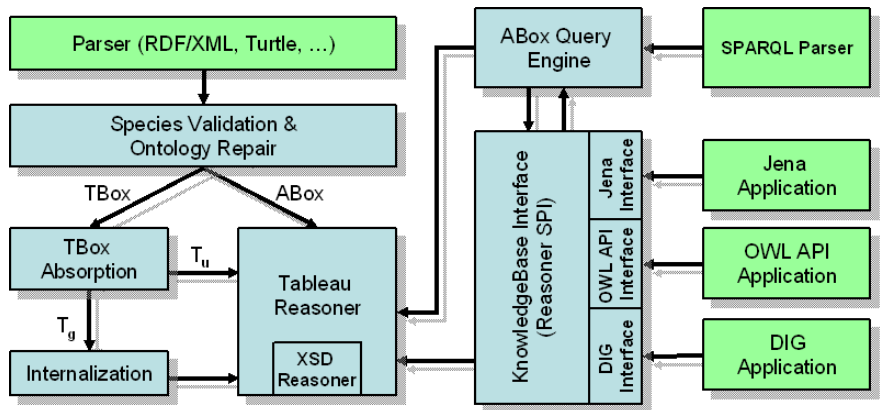
\includegraphics{bilder/pellet_komponenten.png}}}
\caption{Hauptkomponenten des Pellet-Reasoners.\label{fig:pellet_komponenten}\protect\footnotemark}
\end{figure}
\footnotetext{\cite[S. 6]{sirin:pellet05}}

\subsubsection{Beschreibungslogik}
\label{subsubsection:beschreibungslogik}
Beschreibungslogiken sind Formalismen um Wissen darzustellen, dabei sind sie eine Teilmenge der Prädikatenlogik. Sie stellen den Kern von Wissensrepräsentationssystemen dar, in dem sie eine Struktur für eine Wissensbasis und den damit verbundenen Methoden zur Folgerung bieten (vgl.~\cite{dl:baader2003}).

Die Struktur, welche Beschreibungslogiken als Wissensbasis bereitstellen, besteht aus einem Schema (Tbox, Regeln), sowie aus den Daten (Abox, Fakten).

Die Semantik von Beschreibungslogiken wird durch Interpretationen definiert:

\noindent\hspace*{16mm} $ I = (\Delta^I, \cdot^I) $

Dabei ist:
\begin{itemize}
\item $ \Delta^I $

    Die (Wissens-) Domäne (eine nicht leere Menge).

\item $ \cdot^I $

    Eine Funktion zur Interpretation von:
    \begin{itemize}
        \item Konzepten (Klassen, A)

            Wobei $ A^I $ eine Teilmenge von $ \Delta^I $ ist.
        \item Rollen (Eigenschaften, R)

            Wobei $ R^I $ eine binäre Relation auf $ \Delta^I $ ist.
        \item Individuen (i)

            Wobei $ i^I $ Element von $ \Delta^I $ ist.
    \end{itemize}
\end{itemize}

Die Funktion zur (Wissens-) Interpretation $ \cdot^I $ definiert, wie atomare Konzpte, Eigenschaften und Individuen zu interpretieren sind. Eine Interpretation, welche allen Axiomen einer Ontologie in Beschreibungslogik genügt ist ein Modell der Ontologie.

Eine Ontologie in Beschreibungslogik ist eine Menge von Termen und deren Relationen. Die Interpretation dieser Ontologie stellt als ein Modell dar, welches die Ontologie abbildet.

Die Pellet zu Grunde liegende Beschreibungslogik SHOIN (D) ist ein Kürzel und steht für:
\begin{itemize}
\item \textit{S}

ALC (Attributive Concept Language with Complements) mit einer transitiven Rolle. Bei ALC handelt es sich um die kleinste Beschreibungslogik, welche aussagenlogisch geschlossen ist (d.h.\ sie bietet, entweder implizit oder explizit, Konjunktion, Union und Negation von Klassen (-beschreibungen)). Eine Rolle entspricht einer Eigenschaft bzw.\ einem Prädikat in der Prädikatenlogik erster Stufe.

\item \textit{H}

    Rollenhierarchie (Sub-Eigenschaften), z.B. rdfs:subPropertyOf.

\item \textit{O}

    Nominal, z.B. Wochenden = {Samstag, Sonntag}.


\item \textit{I}

    Inverse Rolle (inverse Eigenschaft bzw.\ Prädikt).

\item \textit{N}

    Nummerische Einschränkung, z.B. >= hatKind 1.

\item \textit{(D)}

    Nutzung von Wertebereichen, Werten oder Datentypen.
\end{itemize}

(vgl.~\cite{dl:baader2003})

\subsubsection{Folgerung}
\label{subsubsection:folgerung}
Die W3C Spezifikation betreffend der Umsetzung eines Reasoners definiert zwei Arten von OWL Dokumentprüfungen: Prüfung auf korrekte Syntax sowie Prüfung der Konsistenz. Bei der Konsistenzprüfung geht es darum festzustellen, ob eine gegebene Eingabe anhand einer definierten Spezifikation syntaktisch korrekt ist. Jedoch macht eine reine Umsetzung der genannten Prüfungen wenig Sinn. Man möchte ja eine Ontologie möglichst effektiv nutzen können, zum Beispiel um indirektes Wissen abzuleiten.  Da OWL DL eine syntaktische Variante der Beschreibungslogik SHOIN (D) darstellt, liegt es nahe, mittels einem Reasoner folgende Methoden zur Inferenz zur Verfügung zu stellen:
\begin{itemize}
\item \textit{Konsistenzprüfung}

Stellt sicher, dass sich in der Ontologie keine gegenstätzlichen Fakten befinden. Konkret bedeutet dies anhand der OWL Semantik~\footnote{http://www.w3.org/TR/owl-semantics/}, dass die Konsistenz einer ABox in Bezug auf eine TBox geprüft wird.
\item \textit{Konzept-Erfüllbarkeit}

Stellt sicher, dass Objekte einer Klasse instanziert werden können. Ist dies nicht der Fall, so ist die Ontologie inkonsistent.
\item \textit{Klassifikation}

Berechnet die Relationen zwischen Subklassen, stellt also die Klassenhierarchie auf. Dies ermöglicht das Abfragen der Ontologie.
\item \textit{Gewinnung von Erkenntnissen}

Findet die spezifischste Klasse eines Objektes, leitet also den direkten Typ jedes Objektes ab.
\end{itemize}
(vgl. \citet[S. 1 und 2]{sirin:pellet05})

Bei der eigentliche Komponente, welche in Pellet zur Folgerung eingesetzt wird, handelt es sich um den Tableau Reasoner, welcher den gleichnamigen Algorithmus verwendet. Dieser reduziert ein Problem der Folgerung auf ein Problem der Konzept-Erfüllbarkeit, wobei er eine Interpretation sucht, welche die gefragten Konzepte erfüllt. Solch eine Interpretation wird inkrementell als eine Art Tafel (eben, Tableau) aufgebaut.

Nachfolgend ein Beispiel, gegeben sei:
$ Prolog \subseteq LogischeProgrammiersprache, LogischeProgrammiersprache \subseteq Programmiersprache $
Man stellt nun folgende Anfrage:
$ if Prolog \subseteq Programmiersprache $

Der Prozess der Folgerung findet nun wie folgt statt:
\begin{itemize}
    \item Testen, ob ein Individuum existiert, welches eine logische Programmiersprache, aber keine Programmiersprache ist. Man möchte also die Erfüllbarkeit des Konzeptes $ C_0 = (Prolog \sqcap \neg Programmiersprache) $ testen.
    \item $ C_0(x) \Rightarrow Prolog(x), (\neg Programmiersprache)(x) $
    \item $ Prolog(x) \Rightarrow LogischeProgrammiersprache(x) $
    \item $ LogischeProgrammiersprache(x) \Rightarrow Programmiersprache(x) $
        $ \Rightarrow $ Konflikt!
\end{itemize}
Wie ersichtlich ist, ist das Konzept $ C_0 $ nicht erfüllbar, die Anfrage $ Prolog \subseteq Programmiersprache $ trifft also innerhalb der gegebenen Ontologie zu. Der Beweis wird mittels Kontradiktion erbracht.

Der generelle Prozess der Folgerung läuft wie folgt ab:
\begin{itemize}
    \item Umwandlung eines Konzeptes bzw.\ der Konzepte in die negierte Normalform (NNF), die Negation $ \neg $ befindet sich vor Konzeptnamen.
    \item Ablegen des umgewandelten Konzeptes als $ C_0 $.

        Der Algorithmus hat also die Datenbasis (Abox) $ A_0 = {C_0(x_0)} $
    \item Regeln zur Transformation auf die Datenbasis (Abox) so weit als möglich anwenden.
    \item Wurde eine gültige Datenbasis (Abox) gefunden, so ist $ C_0 $ erfüllbar.
    \item Wurde keine gültige Datenbasis unter Berücksichtigung aller (Such-) Pfade gefunden, so ist $ C_0 $ nicht erfüllbar.
\end{itemize} (vgl.~\cite{horrocks2002} und~\cite{horrocks2005})



\subsection{Beispiel}
\label{subsec:inferenz_beispiel}

Gegeben seien folgende Datensätze, welche Regeln definieren

\begin{lstlisting}[caption={Aussagentripel bestehend aus Objekt, Prädikat und Subjekt},captionpos=b,label=lst:reasoning_seilpark]
    ``Schweiz hatRegion Solothurn.''
    ``Solothurn hatOrt Balmberg.''
    ``Seilpark istUnterklasseVon Ausflug.''
    ``Seilpark hatStandort Balmberg.''
\end{lstlisting}

definiert.

Unterstützt nun ein Programm Inferenz, z.B. durch einen Reasoner, so kann dieser schlussfolgern, dass der Ausflug \textit{Seilpark} in der Region Solothurn ist (vgl.~\cite[Abschnitt `Examples']{w3inference}).

\newpage

\noindent\rule[1ex]{\textwidth}{1pt}
\begin{wrapfigure}[14]{l}{0.1\textwidth}
    \vspace{-12pt}
    
\includegraphics[width=0.1\textwidth]{bilder/elephant.png}
\end{wrapfigure}
Das unter~\ref{lst:reasoning_seilpark} genannte Beispiel beantwortet genau die unter~\ref{sec:wissensrepFormen_Wissensnetze} gestellte Frage, wie man zum Schluss gelangt, dass das Individuum \textit{Seilpark Balmberg} in der \textit{Region} \textit{Solothurn} ist.

Wie wendet man dies jedoch an? Wie gelangt man effektiv zu dieser Information? Kann dies effektiv durch reine Folgerung erreicht werden?

Die Antwort hierzu lautet ja und nein. Modelliert man die Situation beispielsweise in Protégé und nutzt den Pellet-Reasoner zum Ziehen von Schlüssen, so würde man annehmen, dass dies der Fall ist. Rein von den Möglichkeiten her sollte der Reasoner genau dies bieten. Dies ist jedoch nicht ganz der Fall, wie in der nachfolgenden Grafik ersichtlich ist.

\begin{figure}[H]
\centering \rotatebox{0}{\scalebox{0.5}[0.5]{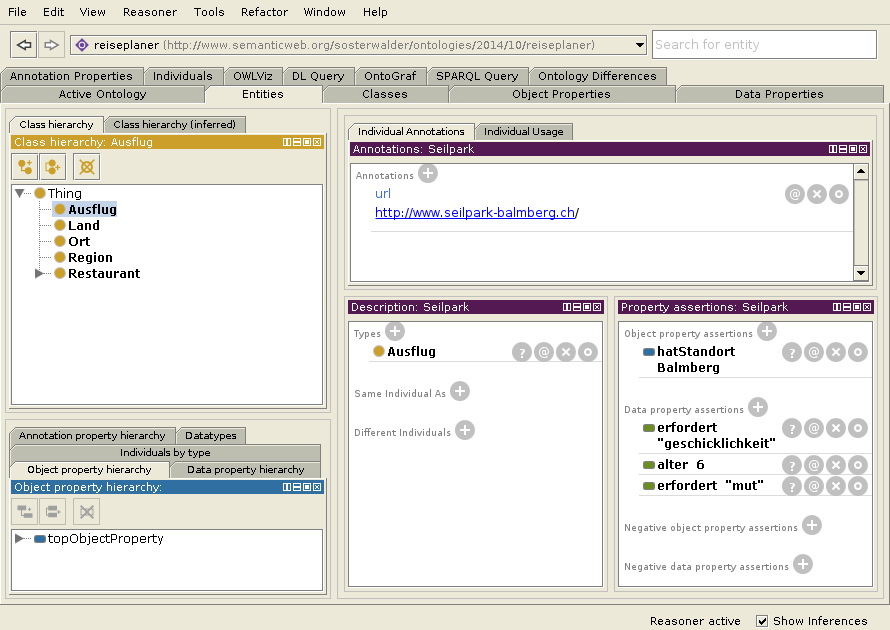
\includegraphics{bilder/inferenz_protege.png}}}
\caption{Darstellung des Individuums \textit{Seilpark Balmberg} in Protégé.\label{fig:inferenz_protege}\protect\footnotemark}
\end{figure}
\footnotetext{Eigene Darstellung mittels Stanford Protégé Version 5.0.0 beta 15}

Eine solche Folgerung ist durchaus möglich, man muss den Relationen die entsprechenden Eigenschaften, wie Symmetrie oder Transivität, geben. Wir haben dies in unserem Fall jedoch bewusst nicht getan, da sonst Folgerungen auftreten, welche irreführend sind, so wäre dann z.B. ein Ort auch ein Land und umgekehrt.

Wir haben die eigentliche Folgerung mittels einer Regel in der Ontologie vorgenommen. Dies führen wir zu einem späteren Zeitpunkt noch genauer aus.

\noindent\rule[1ex]{\textwidth}{1pt}

\subsection{Unterschiede zu Prolog}
\label{}
An dieser Stelle wurden die Unterschiede zwischen Pellet und der Inferenz-Maschine in Prolog ersichtlich. Prolog ist hinsichtlich der Verwendung von Regeln sehr flexibel. So ist man bei der Definition von Regeln nicht eingeschränkt, da diese beliebig viele Fakten und Prädikate enthalten können.

Im Unterschied dazu muss bei der eingesetzten Regelsprache SWRL jedes verwendete Konzept --- Klasse, Individuum, Eigenschaft oder Beziehung --- zuvor definiert werden. Es wird also explizit zwischen den verschiedenen Typen unterschieden. Bei Prolog wird dies nur durch die Menge der Argumente bzw.\ die Argumente selbst definiert.

Ein weiterer, fundamentaler Unterschied ist die Art, wie Schlüsse gezogen werden. Prolog basiert grundsätzlich auf dem SLD-Resolutionsverfahren~\citep[Details siehe][Seite 68]{laemmel}. Im Gegensatz dazu kommt bei dem eingesetzten Reasoner der Tableau-Algorithmus zum Einsatz. Eine Erklärung dieses Algorithmus findet sich im Tutorialdokument unter LINK.

Zusammenfassend kann gesagt werden, dass in Prolog direkt Anfragen gestellt werden können. Rückgabewerte dieser Anfragen sind entweder Wahrheitsaussagen (wahr oder falsch) über Fakten oder aber Objekte bzw. Listen von Objekten. Pellet kann hingegen nur Wahrheitsaussagen treffen. Dies bedeutet, dass Objekten somit nur Eigenschaften zugewiesen werden können, so z.B. die Zugehörigkeit zu einer Klasse, eine Relation zu einem anderen Objekt oder eine Objekteigenschaft (wie Geschlecht, Grösse, Dauer etc.). Die Rückgabe von Objekten findet also nicht durch den Reasoner sondern durch Abfragen, z.B. mittels SPARQL, statt.

So ist es in Prolog ohne Weiteres möglich so genannte Constraint-Satisfaction-Probleme (Bedingungserfüllungsprobleme) zu lösen~\citep[Details siehe][Seite 148]{laemmel}. Mit Pellet bzw. Ontologien und Regeln ist dies nicht ohne Weiteres möglich. Versuche dazu finden sich unter~\citet{xiong2008constraint},~\citet{staab2006constraint} und~\citet{bramer2007constraint}.
